\documentclass[]{article}
\usepackage{lmodern}
\usepackage{amssymb,amsmath}
\usepackage{ifxetex,ifluatex}
\usepackage{fixltx2e} % provides \textsubscript
\ifnum 0\ifxetex 1\fi\ifluatex 1\fi=0 % if pdftex
  \usepackage[T1]{fontenc}
  \usepackage[utf8]{inputenc}
\else % if luatex or xelatex
  \ifxetex
    \usepackage{mathspec}
  \else
    \usepackage{fontspec}
  \fi
  \defaultfontfeatures{Ligatures=TeX,Scale=MatchLowercase}
\fi
% use upquote if available, for straight quotes in verbatim environments
\IfFileExists{upquote.sty}{\usepackage{upquote}}{}
% use microtype if available
\IfFileExists{microtype.sty}{%
\usepackage{microtype}
\UseMicrotypeSet[protrusion]{basicmath} % disable protrusion for tt fonts
}{}
\usepackage[margin=1in]{geometry}
\usepackage{hyperref}
\hypersetup{unicode=true,
            pdftitle={Supplemental Materials \#2: Re-analysis of Study 14 (Monnot et al., 2011) in Yu et al. (2016)},
            pdfauthor={Mike W.-L. Cheung},
            pdfborder={0 0 0},
            breaklinks=true}
\urlstyle{same}  % don't use monospace font for urls
\usepackage{color}
\usepackage{fancyvrb}
\newcommand{\VerbBar}{|}
\newcommand{\VERB}{\Verb[commandchars=\\\{\}]}
\DefineVerbatimEnvironment{Highlighting}{Verbatim}{commandchars=\\\{\}}
% Add ',fontsize=\small' for more characters per line
\usepackage{framed}
\definecolor{shadecolor}{RGB}{248,248,248}
\newenvironment{Shaded}{\begin{snugshade}}{\end{snugshade}}
\newcommand{\KeywordTok}[1]{\textcolor[rgb]{0.13,0.29,0.53}{\textbf{#1}}}
\newcommand{\DataTypeTok}[1]{\textcolor[rgb]{0.13,0.29,0.53}{#1}}
\newcommand{\DecValTok}[1]{\textcolor[rgb]{0.00,0.00,0.81}{#1}}
\newcommand{\BaseNTok}[1]{\textcolor[rgb]{0.00,0.00,0.81}{#1}}
\newcommand{\FloatTok}[1]{\textcolor[rgb]{0.00,0.00,0.81}{#1}}
\newcommand{\ConstantTok}[1]{\textcolor[rgb]{0.00,0.00,0.00}{#1}}
\newcommand{\CharTok}[1]{\textcolor[rgb]{0.31,0.60,0.02}{#1}}
\newcommand{\SpecialCharTok}[1]{\textcolor[rgb]{0.00,0.00,0.00}{#1}}
\newcommand{\StringTok}[1]{\textcolor[rgb]{0.31,0.60,0.02}{#1}}
\newcommand{\VerbatimStringTok}[1]{\textcolor[rgb]{0.31,0.60,0.02}{#1}}
\newcommand{\SpecialStringTok}[1]{\textcolor[rgb]{0.31,0.60,0.02}{#1}}
\newcommand{\ImportTok}[1]{#1}
\newcommand{\CommentTok}[1]{\textcolor[rgb]{0.56,0.35,0.01}{\textit{#1}}}
\newcommand{\DocumentationTok}[1]{\textcolor[rgb]{0.56,0.35,0.01}{\textbf{\textit{#1}}}}
\newcommand{\AnnotationTok}[1]{\textcolor[rgb]{0.56,0.35,0.01}{\textbf{\textit{#1}}}}
\newcommand{\CommentVarTok}[1]{\textcolor[rgb]{0.56,0.35,0.01}{\textbf{\textit{#1}}}}
\newcommand{\OtherTok}[1]{\textcolor[rgb]{0.56,0.35,0.01}{#1}}
\newcommand{\FunctionTok}[1]{\textcolor[rgb]{0.00,0.00,0.00}{#1}}
\newcommand{\VariableTok}[1]{\textcolor[rgb]{0.00,0.00,0.00}{#1}}
\newcommand{\ControlFlowTok}[1]{\textcolor[rgb]{0.13,0.29,0.53}{\textbf{#1}}}
\newcommand{\OperatorTok}[1]{\textcolor[rgb]{0.81,0.36,0.00}{\textbf{#1}}}
\newcommand{\BuiltInTok}[1]{#1}
\newcommand{\ExtensionTok}[1]{#1}
\newcommand{\PreprocessorTok}[1]{\textcolor[rgb]{0.56,0.35,0.01}{\textit{#1}}}
\newcommand{\AttributeTok}[1]{\textcolor[rgb]{0.77,0.63,0.00}{#1}}
\newcommand{\RegionMarkerTok}[1]{#1}
\newcommand{\InformationTok}[1]{\textcolor[rgb]{0.56,0.35,0.01}{\textbf{\textit{#1}}}}
\newcommand{\WarningTok}[1]{\textcolor[rgb]{0.56,0.35,0.01}{\textbf{\textit{#1}}}}
\newcommand{\AlertTok}[1]{\textcolor[rgb]{0.94,0.16,0.16}{#1}}
\newcommand{\ErrorTok}[1]{\textcolor[rgb]{0.64,0.00,0.00}{\textbf{#1}}}
\newcommand{\NormalTok}[1]{#1}
\usepackage{graphicx,grffile}
\makeatletter
\def\maxwidth{\ifdim\Gin@nat@width>\linewidth\linewidth\else\Gin@nat@width\fi}
\def\maxheight{\ifdim\Gin@nat@height>\textheight\textheight\else\Gin@nat@height\fi}
\makeatother
% Scale images if necessary, so that they will not overflow the page
% margins by default, and it is still possible to overwrite the defaults
% using explicit options in \includegraphics[width, height, ...]{}
\setkeys{Gin}{width=\maxwidth,height=\maxheight,keepaspectratio}
\IfFileExists{parskip.sty}{%
\usepackage{parskip}
}{% else
\setlength{\parindent}{0pt}
\setlength{\parskip}{6pt plus 2pt minus 1pt}
}
\setlength{\emergencystretch}{3em}  % prevent overfull lines
\providecommand{\tightlist}{%
  \setlength{\itemsep}{0pt}\setlength{\parskip}{0pt}}
\setcounter{secnumdepth}{0}
% Redefines (sub)paragraphs to behave more like sections
\ifx\paragraph\undefined\else
\let\oldparagraph\paragraph
\renewcommand{\paragraph}[1]{\oldparagraph{#1}\mbox{}}
\fi
\ifx\subparagraph\undefined\else
\let\oldsubparagraph\subparagraph
\renewcommand{\subparagraph}[1]{\oldsubparagraph{#1}\mbox{}}
\fi

%%% Use protect on footnotes to avoid problems with footnotes in titles
\let\rmarkdownfootnote\footnote%
\def\footnote{\protect\rmarkdownfootnote}

%%% Change title format to be more compact
\usepackage{titling}

% Create subtitle command for use in maketitle
\newcommand{\subtitle}[1]{
  \posttitle{
    \begin{center}\large#1\end{center}
    }
}

\setlength{\droptitle}{-2em}

  \title{Supplemental Materials \#2: Re-analysis of Study 14 (Monnot et al.,
2011) in Yu et al. (2016)}
    \pretitle{\vspace{\droptitle}\centering\huge}
  \posttitle{\par}
    \author{Mike W.-L. Cheung}
    \preauthor{\centering\large\emph}
  \postauthor{\par}
      \predate{\centering\large\emph}
  \postdate{\par}
    \date{July 13, 2018}


\begin{document}
\maketitle

{
\setcounter{tocdepth}{2}
\tableofcontents
}
\section{Functions for the analysis}\label{functions-for-the-analysis}

\begin{itemize}
\tightlist
\item
  This function is modified from the one in Yu et al. (2016)
  Supplemental Materials \#1 with three key differences:

  \begin{enumerate}
  \def\labelenumi{\arabic{enumi}.}
  \tightlist
  \item
    The original function incorrectly uses SDs to represent variances to
    generate the bootstrap correlation matrices. This error is corrected
    here.
  \item
    The original function calls build.matrix() recursively. R will throw
    an error when it goes too deep in generating positive definite
    matrices. This revised function breaks it down into two functions so
    that there are no recursive calls.
  \item
    It adds a \texttt{nearPD} argument. If it is \texttt{TRUE}, it
    transforms the non-positive definite matrices into the near positive
    definite matrices with the \texttt{nearPD()} function in the
    \texttt{Matrix} package. If it is \texttt{FALSE}, new matrices will
    be generated until it is positive definite.
  \end{enumerate}
\end{itemize}

\begin{Shaded}
\begin{Highlighting}[]
\NormalTok{random.matrices <-}\StringTok{ }\ControlFlowTok{function}\NormalTok{(point.matrix, reps, }\DataTypeTok{nearPD=}\OtherTok{FALSE}\NormalTok{) \{}
\NormalTok{  ## SDs of the correlations}
\NormalTok{  SDs <-}\StringTok{ }\KeywordTok{diag}\NormalTok{(point.matrix[,,}\DecValTok{2}\NormalTok{][}\KeywordTok{lower.tri}\NormalTok{(point.matrix[,,}\DecValTok{2}\NormalTok{])])}

\NormalTok{  ## Convert the SDs to Variances}
\NormalTok{  sigma <-}\StringTok{ }\NormalTok{SDs}\OperatorTok{^}\DecValTok{2}
  
\NormalTok{  ## Mean of correlation vector}
\NormalTok{  mu <-}\StringTok{ }\NormalTok{point.matrix[,,}\DecValTok{1}\NormalTok{][}\KeywordTok{lower.tri}\NormalTok{(point.matrix[,,}\DecValTok{1}\NormalTok{])]}
    
\NormalTok{  build.matrix <-}\StringTok{ }\ControlFlowTok{function}\NormalTok{(mu, sigma)  \{}
\NormalTok{    vec <-}\StringTok{ }\KeywordTok{mvrnorm}\NormalTok{(}\DecValTok{1}\NormalTok{, mu, }\DataTypeTok{Sigma=}\NormalTok{sigma )}
\NormalTok{    mat <-}\StringTok{ }\KeywordTok{diag}\NormalTok{(}\DecValTok{1}\NormalTok{, }\KeywordTok{nrow}\NormalTok{(point.matrix))}
\NormalTok{    mat[}\KeywordTok{lower.tri}\NormalTok{(mat)] <-}\StringTok{ }\NormalTok{vec}
\NormalTok{    trans.mat <-}\StringTok{ }\KeywordTok{t}\NormalTok{(mat)}
\NormalTok{    mat[}\KeywordTok{upper.tri}\NormalTok{(mat)] <-}\StringTok{ }\NormalTok{trans.mat[}\KeywordTok{upper.tri}\NormalTok{(trans.mat)]}
\NormalTok{    mat}
\NormalTok{  \}}
 
\NormalTok{  ## Counter for NPD matrices}
\NormalTok{  countNPD <-}\StringTok{ }\DecValTok{0}
  
\NormalTok{  ## Setup an array to store the generated correlation matrices}
\NormalTok{  output <-}\StringTok{ }\KeywordTok{array}\NormalTok{(}\DecValTok{1}\NormalTok{, }\DataTypeTok{dim =} \KeywordTok{c}\NormalTok{(}\KeywordTok{nrow}\NormalTok{(point.matrix), }\KeywordTok{ncol}\NormalTok{(point.matrix), reps))}
  
  \ControlFlowTok{for}\NormalTok{ (rep }\ControlFlowTok{in} \DecValTok{1}\OperatorTok{:}\NormalTok{reps) \{ }
\NormalTok{    mat <-}\StringTok{ }\KeywordTok{build.matrix}\NormalTok{(}\DataTypeTok{mu=}\NormalTok{mu, }\DataTypeTok{sigma=}\NormalTok{sigma)}
    
\NormalTok{    ## Run nearPD==TRUE}
    \ControlFlowTok{if}\NormalTok{ (nearPD) \{}
      \ControlFlowTok{if}\NormalTok{ (}\OperatorTok{!}\KeywordTok{is.positive.definite}\NormalTok{(mat)) \{}
\NormalTok{        mat <-}\StringTok{ }\KeywordTok{as.matrix}\NormalTok{(}\KeywordTok{nearPD}\NormalTok{(mat, }\DataTypeTok{keepDiag =}\NormalTok{ T)}\OperatorTok{$}\NormalTok{mat)}
\NormalTok{        countNPD <-}\StringTok{ }\NormalTok{countNPD}\OperatorTok{+}\DecValTok{1}
\NormalTok{      \}}
\NormalTok{    \} }\ControlFlowTok{else}\NormalTok{ \{}
\NormalTok{      ## Run rearPD==FALSE}
      \ControlFlowTok{while}\NormalTok{(}\OperatorTok{!}\KeywordTok{is.positive.definite}\NormalTok{(mat)) \{}
\NormalTok{        mat <-}\StringTok{ }\KeywordTok{build.matrix}\NormalTok{(}\DataTypeTok{mu=}\NormalTok{mu, }\DataTypeTok{sigma=}\NormalTok{sigma)}
\NormalTok{        countNPD <-}\StringTok{ }\NormalTok{countNPD}\OperatorTok{+}\DecValTok{1}
\NormalTok{      \} }
\NormalTok{    \}}
    
\NormalTok{    output[,,rep] <-}\StringTok{ }\NormalTok{mat}
\NormalTok{  \}}
  \KeywordTok{rownames}\NormalTok{(output) <-}\StringTok{ }\KeywordTok{colnames}\NormalTok{(output) <-}\StringTok{ }\KeywordTok{rownames}\NormalTok{(point.matrix)}
  \KeywordTok{return}\NormalTok{(}\KeywordTok{list}\NormalTok{(}\DataTypeTok{countTotal=}\NormalTok{(reps}\OperatorTok{+}\NormalTok{countNPD), }\DataTypeTok{countNPD=}\NormalTok{countNPD, }\DataTypeTok{data=}\NormalTok{output))}
\NormalTok{\}}


\NormalTok{## This function tests the biases of the generated data.}
\NormalTok{testBias <-}\StringTok{ }\ControlFlowTok{function}\NormalTok{(point.matrix, reps, }\DataTypeTok{nearPD=}\OtherTok{FALSE}\NormalTok{) \{}
\NormalTok{  ## Generate data}
\NormalTok{  mat <-}\StringTok{ }\KeywordTok{random.matrices}\NormalTok{(}\DataTypeTok{point.matrix=}\NormalTok{point.matrix, }\DataTypeTok{reps=}\NormalTok{reps, }\DataTypeTok{nearPD=}\NormalTok{nearPD)}
  
\NormalTok{  ## Convert it into a list for ease of manipulations}
\NormalTok{  mat.list <-}\StringTok{ }\KeywordTok{alply}\NormalTok{(mat}\OperatorTok{$}\NormalTok{data, }\DecValTok{3}\NormalTok{)}

\NormalTok{  ## Percentage of matrices is PD}
\NormalTok{  Percentage.NPD <-}\StringTok{ }\NormalTok{mat}\OperatorTok{$}\NormalTok{countNPD}\OperatorTok{/}\NormalTok{mat}\OperatorTok{$}\NormalTok{countTotal}\OperatorTok{*}\DecValTok{100}
  
\NormalTok{  ## Convert the list into a matrix of vectors to calculate mean and SD}
\NormalTok{  mat.vec <-}\StringTok{ }\KeywordTok{t}\NormalTok{(}\KeywordTok{sapply}\NormalTok{(mat.list, lav_matrix_vech, }\DataTypeTok{diagonal=}\OtherTok{FALSE}\NormalTok{))}
  
\NormalTok{  ## Mean of the correlation matrices}
\NormalTok{  mat.rc <-}\StringTok{ }\KeywordTok{lav_matrix_vech_reverse}\NormalTok{(}\KeywordTok{apply}\NormalTok{(mat.vec, }\DecValTok{2}\NormalTok{, mean), }\DataTypeTok{diagonal =} \OtherTok{FALSE}\NormalTok{)}
  \KeywordTok{diag}\NormalTok{(mat.rc) <-}\StringTok{ }\DecValTok{1}

  \CommentTok{# Percentage bias of the mean}
\NormalTok{  Percentage.bias.rc <-}\StringTok{ }\NormalTok{(mat.rc}\OperatorTok{-}\NormalTok{point.matrix[,,}\DecValTok{1}\NormalTok{])}\OperatorTok{/}\NormalTok{point.matrix[,,}\DecValTok{1}\NormalTok{]}\OperatorTok{*}\DecValTok{100}
  \CommentTok{# Remove Inf as NA}
\NormalTok{  Percentage.bias.rc[}\KeywordTok{is.infinite}\NormalTok{(Percentage.bias.rc)] <-}\StringTok{ }\OtherTok{NA}
  
\NormalTok{  ## sd of the correlation matrices}
\NormalTok{  mat.sd <-}\StringTok{ }\KeywordTok{lav_matrix_vech_reverse}\NormalTok{(}\KeywordTok{apply}\NormalTok{(mat.vec, }\DecValTok{2}\NormalTok{, sd), }\DataTypeTok{diagonal =} \OtherTok{FALSE}\NormalTok{)}
  
  \CommentTok{# Percentage bias of the SDs}
\NormalTok{  Percentage.bias.sd <-}\StringTok{ }\NormalTok{(mat.sd}\OperatorTok{-}\NormalTok{point.matrix[,,}\DecValTok{2}\NormalTok{])}\OperatorTok{/}\NormalTok{point.matrix[,,}\DecValTok{2}\NormalTok{]}\OperatorTok{*}\DecValTok{100}
  
\NormalTok{  ## Bias of correlation among the generated correlation vectors}
\NormalTok{  CorAmongCor <-}\StringTok{ }\KeywordTok{lav_matrix_vech}\NormalTok{(}\KeywordTok{cor}\NormalTok{(mat.vec), }\DataTypeTok{diagonal =} \OtherTok{FALSE}\NormalTok{)}

  \KeywordTok{list}\NormalTok{(}\DataTypeTok{summary=}\KeywordTok{list}\NormalTok{(}\DataTypeTok{Percentage.NPD=}\NormalTok{Percentage.NPD, }
                    \DataTypeTok{Percentage.bias.rc=}\NormalTok{Percentage.bias.rc,}
                    \DataTypeTok{Percentage.bias.sd=}\NormalTok{Percentage.bias.sd,}
      \DataTypeTok{Summary.percentage.bias.rc=}\KeywordTok{summary}\NormalTok{(}\KeywordTok{lav_matrix_vech}\NormalTok{(Percentage.bias.rc, }\DataTypeTok{diagonal =} \OtherTok{FALSE}\NormalTok{)),}
      \DataTypeTok{Summary.percentage.bias.sd=}\KeywordTok{summary}\NormalTok{(}\KeywordTok{lav_matrix_vech}\NormalTok{(Percentage.bias.sd, }\DataTypeTok{diagonal =} \OtherTok{FALSE}\NormalTok{)),}
                    \DataTypeTok{CorAmongCor=}\KeywordTok{summary}\NormalTok{(CorAmongCor)), }\DataTypeTok{data=}\NormalTok{mat}\OperatorTok{$}\NormalTok{data)}
\NormalTok{\}}

\NormalTok{## This function is based on the one in Yu et al. Supplemental Materials #1}
\NormalTok{FIMASEM <-}\StringTok{ }\ControlFlowTok{function}\NormalTok{(model, input.matrices, sample.nobs) \{}
\NormalTok{  coefs.fits <-}\StringTok{ }\KeywordTok{as.data.frame}\NormalTok{(}\KeywordTok{t}\NormalTok{(}\KeywordTok{sapply}\NormalTok{(}\DecValTok{1}\OperatorTok{:}\KeywordTok{dim}\NormalTok{(input.matrices)[}\DecValTok{3}\NormalTok{], }\ControlFlowTok{function}\NormalTok{(i) \{}
\NormalTok{    temp.sem <-}\StringTok{ }\KeywordTok{sem}\NormalTok{(}\DataTypeTok{model=}\NormalTok{model, }\DataTypeTok{sample.nobs=}\NormalTok{sample.nobs,}
                    \DataTypeTok{sample.cov=}\NormalTok{input.matrices[,,i], }\DataTypeTok{warn=}\OtherTok{FALSE}\NormalTok{)}
    \KeywordTok{c}\NormalTok{(}\KeywordTok{coef}\NormalTok{(temp.sem), }\KeywordTok{fitMeasures}\NormalTok{(temp.sem))\})))}
\NormalTok{\}}
\end{Highlighting}
\end{Shaded}

\section{Input data}\label{input-data}

\begin{Shaded}
\begin{Highlighting}[]
\NormalTok{## Required packages}
\NormalTok{lib2install <-}\StringTok{ }\KeywordTok{c}\NormalTok{(}\StringTok{"plyr"}\NormalTok{, }\StringTok{"matrixcalc"}\NormalTok{, }\StringTok{"lavaan"}\NormalTok{, }\StringTok{"MASS"}\NormalTok{, }\StringTok{"psych"}\NormalTok{, }\StringTok{"Matrix"}\NormalTok{)}

\NormalTok{## Install them automatically if they are not available on your computer}
\ControlFlowTok{for}\NormalTok{ (i }\ControlFlowTok{in}\NormalTok{ lib2install) \{}
  \ControlFlowTok{if}\NormalTok{ (}\OperatorTok{!}\NormalTok{(i }\OperatorTok\StringTok{ }\KeywordTok{rownames}\NormalTok{(}\KeywordTok{installed.packages}\NormalTok{()))) }\KeywordTok{install.packages}\NormalTok{(i)}
\NormalTok{\}}

\NormalTok{## Libraries used in the analysis}
\KeywordTok{library}\NormalTok{(plyr)}
\KeywordTok{library}\NormalTok{(matrixcalc)}
\KeywordTok{library}\NormalTok{(lavaan)}
\KeywordTok{library}\NormalTok{(MASS)}
\KeywordTok{library}\NormalTok{(psych)  }
\KeywordTok{library}\NormalTok{(Matrix)}

\NormalTok{## Set the seed for replication}
\KeywordTok{set.seed}\NormalTok{(}\DecValTok{927037462}\NormalTok{)}

\NormalTok{## Large bootstrap replications to minimize simulation error}
\NormalTok{reps <-}\StringTok{ }\DecValTok{10000}

\NormalTok{## Sample size}
\NormalTok{sample.nobs <-}\StringTok{ }\DecValTok{200}
\end{Highlighting}
\end{Shaded}

\begin{itemize}
\tightlist
\item
  It is important to note that standard deviations (SDs) were
  incorrectly used to represent variances to generate the bootstrap
  correlation matrices in the \texttt{random.matrices.univarite()} in
  Yu's et al. Supplemental Materials \#1. This error is corrected here.

  \begin{itemize}
  \tightlist
  \item
    \texttt{inputmatrices}: SD matrix used in Yu et al. (2016)
  \end{itemize}
\end{itemize}

\begin{Shaded}
\begin{Highlighting}[]
\NormalTok{rc <-}\StringTok{ }\KeywordTok{matrix}\NormalTok{(}\KeywordTok{c}\NormalTok{(}\DecValTok{1}\NormalTok{,.}\DecValTok{47}\NormalTok{,.}\DecValTok{12}\NormalTok{,.}\DecValTok{20}\NormalTok{,.}\DecValTok{24}\NormalTok{,.}\DecValTok{00}\NormalTok{,}
\NormalTok{               .}\DecValTok{47}\NormalTok{,}\DecValTok{1}\NormalTok{,.}\DecValTok{11}\NormalTok{,.}\DecValTok{18}\NormalTok{,.}\DecValTok{11}\NormalTok{,}\OperatorTok{-}\NormalTok{.}\DecValTok{04}\NormalTok{,}
\NormalTok{               .}\DecValTok{12}\NormalTok{,.}\DecValTok{11}\NormalTok{,}\DecValTok{1}\NormalTok{,.}\DecValTok{70}\NormalTok{,.}\DecValTok{73}\NormalTok{,.}\DecValTok{40}\NormalTok{,}
\NormalTok{               .}\DecValTok{20}\NormalTok{,.}\DecValTok{18}\NormalTok{,.}\DecValTok{70}\NormalTok{,}\DecValTok{1}\NormalTok{,.}\DecValTok{56}\NormalTok{,.}\DecValTok{22}\NormalTok{,}
\NormalTok{               .}\DecValTok{24}\NormalTok{,.}\DecValTok{11}\NormalTok{,.}\DecValTok{73}\NormalTok{,.}\DecValTok{56}\NormalTok{,}\DecValTok{1}\NormalTok{,.}\DecValTok{41}\NormalTok{,}
\NormalTok{               .}\DecValTok{00}\NormalTok{,}\OperatorTok{-}\NormalTok{.}\DecValTok{04}\NormalTok{,.}\DecValTok{40}\NormalTok{,.}\DecValTok{22}\NormalTok{,.}\DecValTok{41}\NormalTok{,}\DecValTok{1}\NormalTok{), }\DataTypeTok{nr=}\DecValTok{6}\NormalTok{)}
\NormalTok{sd <-}\StringTok{ }\KeywordTok{matrix}\NormalTok{(}\KeywordTok{c}\NormalTok{(.}\DecValTok{00}\NormalTok{,.}\DecValTok{30}\NormalTok{,.}\DecValTok{20}\NormalTok{,.}\DecValTok{14}\NormalTok{,.}\DecValTok{23}\NormalTok{,.}\DecValTok{20}\NormalTok{,}
\NormalTok{              .}\DecValTok{30}\NormalTok{,.}\DecValTok{00}\NormalTok{,.}\DecValTok{22}\NormalTok{,.}\DecValTok{17}\NormalTok{,.}\DecValTok{22}\NormalTok{,.}\DecValTok{18}\NormalTok{,}
\NormalTok{              .}\DecValTok{20}\NormalTok{,.}\DecValTok{22}\NormalTok{,.}\DecValTok{00}\NormalTok{,.}\DecValTok{19}\NormalTok{,.}\DecValTok{16}\NormalTok{,.}\DecValTok{20}\NormalTok{,}
\NormalTok{              .}\DecValTok{14}\NormalTok{,.}\DecValTok{17}\NormalTok{,.}\DecValTok{19}\NormalTok{,.}\DecValTok{00}\NormalTok{,.}\DecValTok{26}\NormalTok{,.}\DecValTok{16}\NormalTok{,}
\NormalTok{              .}\DecValTok{23}\NormalTok{,.}\DecValTok{22}\NormalTok{,.}\DecValTok{16}\NormalTok{,.}\DecValTok{26}\NormalTok{,}\DecValTok{0}\NormalTok{,.}\DecValTok{24}\NormalTok{,}
\NormalTok{              .}\DecValTok{20}\NormalTok{,.}\DecValTok{18}\NormalTok{,.}\DecValTok{20}\NormalTok{,.}\DecValTok{16}\NormalTok{,.}\DecValTok{24}\NormalTok{,}\DecValTok{0}\NormalTok{), }\DataTypeTok{nr=}\DecValTok{6}\NormalTok{)}
\NormalTok{input.matrices <-}\StringTok{ }\KeywordTok{array}\NormalTok{(}\DecValTok{0}\NormalTok{, }\DataTypeTok{dim=}\KeywordTok{c}\NormalTok{(}\KeywordTok{nrow}\NormalTok{(rc), }\KeywordTok{ncol}\NormalTok{(rc),}\DecValTok{2}\NormalTok{))}
\NormalTok{input.matrices[,,}\DecValTok{1}\NormalTok{] <-}\StringTok{ }\NormalTok{rc}
\NormalTok{input.matrices[,,}\DecValTok{2}\NormalTok{] <-}\StringTok{ }\NormalTok{sd}
\KeywordTok{dimnames}\NormalTok{(input.matrices) <-}\StringTok{ }\KeywordTok{list}\NormalTok{(}\KeywordTok{c}\NormalTok{(}\StringTok{'ORGC'}\NormalTok{,}\StringTok{'JSAT'}\NormalTok{,}\StringTok{'PROUATT'}\NormalTok{,}\StringTok{'INSTRU'}\NormalTok{,}\StringTok{'UCOM'}\NormalTok{,}\StringTok{'UPART'}\NormalTok{),}
                                 \KeywordTok{c}\NormalTok{(}\StringTok{'ORGC'}\NormalTok{,}\StringTok{'JSAT'}\NormalTok{,}\StringTok{'PROUATT'}\NormalTok{,}\StringTok{'INSTRU'}\NormalTok{,}\StringTok{'UCOM'}\NormalTok{,}\StringTok{'UPART'}\NormalTok{),}
                                 \KeywordTok{c}\NormalTok{(}\StringTok{"rc"}\NormalTok{, }\StringTok{"sd"}\NormalTok{))}
\NormalTok{input.matrices}
\end{Highlighting}
\end{Shaded}

\begin{verbatim}
## , , rc
## 
##         ORGC  JSAT PROUATT INSTRU UCOM UPART
## ORGC    1.00  0.47    0.12   0.20 0.24  0.00
## JSAT    0.47  1.00    0.11   0.18 0.11 -0.04
## PROUATT 0.12  0.11    1.00   0.70 0.73  0.40
## INSTRU  0.20  0.18    0.70   1.00 0.56  0.22
## UCOM    0.24  0.11    0.73   0.56 1.00  0.41
## UPART   0.00 -0.04    0.40   0.22 0.41  1.00
## 
## , , sd
## 
##         ORGC JSAT PROUATT INSTRU UCOM UPART
## ORGC    0.00 0.30    0.20   0.14 0.23  0.20
## JSAT    0.30 0.00    0.22   0.17 0.22  0.18
## PROUATT 0.20 0.22    0.00   0.19 0.16  0.20
## INSTRU  0.14 0.17    0.19   0.00 0.26  0.16
## UCOM    0.23 0.22    0.16   0.26 0.00  0.24
## UPART   0.20 0.18    0.20   0.16 0.24  0.00
\end{verbatim}

\section{Checking the generated correlation
matrices}\label{checking-the-generated-correlation-matrices}

\subsection{Replace NPD correlation matrices with newly generated
matrices (replacement
method)}\label{replace-npd-correlation-matrices-with-newly-generated-matrices-replacement-method}

\begin{Shaded}
\begin{Highlighting}[]
\NormalTok{replacement.data <-}\StringTok{ }\KeywordTok{testBias}\NormalTok{(}\DataTypeTok{point.matrix=}\NormalTok{input.matrices, }\DataTypeTok{reps=}\NormalTok{reps, }\DataTypeTok{nearPD=}\OtherTok{FALSE}\NormalTok{)}
\NormalTok{replacement.data}\OperatorTok{$}\NormalTok{summary}
\end{Highlighting}
\end{Shaded}

\begin{verbatim}
## $Percentage.NPD
## [1] 74.72066
## 
## $Percentage.bias.rc
##                ORGC        JSAT     PROUATT      INSTRU       UCOM
## ORGC      0.0000000 -20.3546341  13.9482931  -0.8136603 -14.486557
## JSAT    -20.3546341   0.0000000   0.6180548  -2.7104838   5.806848
## PROUATT  13.9482931   0.6180548   0.0000000 -11.5333205 -10.058401
## INSTRU   -0.8136603  -2.7104838 -11.5333205   0.0000000  -6.821452
## UCOM    -14.4865571   5.8068476 -10.0584013  -6.8214520   0.000000
## UPART            NA -12.9549677  -5.8898993   5.8309321 -10.331016
##              UPART
## ORGC            NA
## JSAT    -12.954968
## PROUATT  -5.889899
## INSTRU    5.830932
## UCOM    -10.331016
## UPART     0.000000
## 
## $Percentage.bias.sd
##               ORGC       JSAT   PROUATT     INSTRU      UCOM      UPART
## ORGC           NaN -18.655245 -13.56228  -5.383758 -15.83886  -5.357794
## JSAT    -18.655245        NaN -15.14714  -6.172967 -13.04984  -5.104401
## PROUATT -13.562278 -15.147142       NaN -22.546825 -19.97234 -13.962333
## INSTRU   -5.383758  -6.172967 -22.54683        NaN -27.39910  -6.051394
## UCOM    -15.838856 -13.049844 -19.97234 -27.399097       NaN -17.534838
## UPART    -5.357794  -5.104401 -13.96233  -6.051394 -17.53484        NaN
## 
## $Summary.percentage.bias.rc
##     Min.  1st Qu.   Median     Mean  3rd Qu.     Max.     NA's 
## -20.3546 -11.2327  -6.3557  -4.9822   0.2601  13.9483        1 
## 
## $Summary.percentage.bias.sd
##    Min. 1st Qu.  Median    Mean 3rd Qu.    Max. 
## -27.399 -18.095 -13.962 -13.716  -6.112  -5.104 
## 
## $CorAmongCor
##       Min.    1st Qu.     Median       Mean    3rd Qu.       Max. 
## -0.0646523 -0.0153979 -0.0006046  0.0120218  0.0200958  0.1617657
\end{verbatim}

\subsection{Replace NPD correlation matrices with nearPD matrices
(nearPD
method)}\label{replace-npd-correlation-matrices-with-nearpd-matrices-nearpd-method}

\begin{Shaded}
\begin{Highlighting}[]
\NormalTok{nearPD.data <-}\StringTok{ }\KeywordTok{testBias}\NormalTok{(}\DataTypeTok{point.matrix=}\NormalTok{input.matrices, }\DataTypeTok{reps=}\NormalTok{reps, }\DataTypeTok{nearPD=}\OtherTok{TRUE}\NormalTok{)}
\NormalTok{nearPD.data}\OperatorTok{$}\NormalTok{summary}
\end{Highlighting}
\end{Shaded}

\begin{verbatim}
## $Percentage.NPD
## [1] 43.20763
## 
## $Percentage.bias.rc
##               ORGC         JSAT     PROUATT     INSTRU      UCOM
## ORGC     0.0000000  -4.20810649  8.24636236 -0.6371194 -5.498776
## JSAT    -4.2081065   0.00000000  0.02210231 -1.8611796  2.847520
## PROUATT  8.2463624   0.02210231  0.00000000 -4.3695688 -4.777884
## INSTRU  -0.6371194  -1.86117956 -4.36956885  0.0000000 -1.369934
## UCOM    -5.4987756   2.84752011 -4.77788410 -1.3699339  0.000000
## UPART           NA -11.32082825 -1.08899926  3.6836698 -2.805620
##              UPART
## ORGC            NA
## JSAT    -11.320828
## PROUATT  -1.088999
## INSTRU    3.683670
## UCOM     -2.805620
## UPART     0.000000
## 
## $Percentage.bias.sd
##              ORGC      JSAT    PROUATT     INSTRU       UCOM     UPART
## ORGC          NaN -9.492244  -9.523041  -5.798344  -9.057849 -3.112887
## JSAT    -9.492244       NaN  -9.642144  -6.178509  -8.623723 -4.959597
## PROUATT -9.523041 -9.642144        NaN -16.106709 -18.544962 -8.165233
## INSTRU  -5.798344 -6.178509 -16.106709        NaN -15.341907 -3.775147
## UCOM    -9.057849 -8.623723 -18.544962 -15.341907        NaN -9.140049
## UPART   -3.112887 -4.959597  -8.165233  -3.775147  -9.140049       NaN
## 
## $Summary.percentage.bias.rc
##     Min.  1st Qu.   Median     Mean  3rd Qu.     Max.     NA's 
## -11.3208  -4.3292  -1.6156  -1.6527  -0.1427   8.2464        1 
## 
## $Summary.percentage.bias.sd
##    Min. 1st Qu.  Median    Mean 3rd Qu.    Max. 
## -18.545  -9.583  -9.058  -9.164  -5.988  -3.113 
## 
## $CorAmongCor
##       Min.    1st Qu.     Median       Mean    3rd Qu.       Max. 
## -0.0608334 -0.0113056  0.0008941  0.0104198  0.0237635  0.1451707
\end{verbatim}

\section{Re-analysis of FIMASEM}\label{re-analysis-of-fimasem}

\begin{Shaded}
\begin{Highlighting}[]
\NormalTok{model <-}\StringTok{ "UPART ~ UCOM}
\StringTok{          UCOM ~ ORGC + JSAT + PROUATT + INSTRU}
\StringTok{          ORGC ~ JSAT}
\StringTok{          PROUATT ~ INSTRU"}
\end{Highlighting}
\end{Shaded}

\subsection{Analysis of the bootstrap data with replacement
method}\label{analysis-of-the-bootstrap-data-with-replacement-method}

\begin{Shaded}
\begin{Highlighting}[]
\NormalTok{fit <-}\StringTok{ }\KeywordTok{FIMASEM}\NormalTok{(model, replacement.data}\OperatorTok{$}\NormalTok{data, }\DataTypeTok{sample.nobs=}\NormalTok{sample.nobs)}

\NormalTok{cfi.fit <-}\StringTok{ }\KeywordTok{ifelse}\NormalTok{(fit}\OperatorTok{$}\NormalTok{cfi}\OperatorTok{>}\FloatTok{0.9}\NormalTok{, }\DataTypeTok{yes=}\DecValTok{1}\NormalTok{, }\DataTypeTok{no=}\DecValTok{0}\NormalTok{)}
\NormalTok{srmr.fit <-}\StringTok{ }\KeywordTok{ifelse}\NormalTok{(fit}\OperatorTok{$}\NormalTok{srmr}\OperatorTok{<}\FloatTok{0.1}\NormalTok{, }\DataTypeTok{yes=}\DecValTok{1}\NormalTok{, }\DataTypeTok{no=}\DecValTok{0}\NormalTok{)}
\NormalTok{rmsea.fit <-}\StringTok{ }\KeywordTok{ifelse}\NormalTok{(fit}\OperatorTok{$}\NormalTok{rmsea}\OperatorTok{<}\FloatTok{0.05}\NormalTok{, }\DataTypeTok{yes=}\DecValTok{1}\NormalTok{, }\DataTypeTok{no=}\DecValTok{0}\NormalTok{)}

\KeywordTok{cat}\NormalTok{(}\StringTok{"Percentage of CFA >.9:"}\NormalTok{, }\KeywordTok{mean}\NormalTok{(cfi.fit)}\OperatorTok{*}\DecValTok{100}\NormalTok{)}
\end{Highlighting}
\end{Shaded}

\begin{verbatim}
## Percentage of CFA >.9: 9.71
\end{verbatim}

\begin{Shaded}
\begin{Highlighting}[]
\KeywordTok{cat}\NormalTok{(}\StringTok{"Percentage of SRMR < .1:"}\NormalTok{, }\KeywordTok{mean}\NormalTok{(srmr.fit)}\OperatorTok{*}\DecValTok{100}\NormalTok{)}
\end{Highlighting}
\end{Shaded}

\begin{verbatim}
## Percentage of SRMR < .1: 20.51
\end{verbatim}

\begin{Shaded}
\begin{Highlighting}[]
\KeywordTok{cat}\NormalTok{(}\StringTok{"Percentage of sample RMSEA < .05:"}\NormalTok{, }\KeywordTok{mean}\NormalTok{(rmsea.fit)}\OperatorTok{*}\DecValTok{100}\NormalTok{)}
\end{Highlighting}
\end{Shaded}

\begin{verbatim}
## Percentage of sample RMSEA < .05: 0.07
\end{verbatim}

\begin{Shaded}
\begin{Highlighting}[]
\KeywordTok{describe}\NormalTok{(fit[, }\KeywordTok{c}\NormalTok{(}\StringTok{"chisq"}\NormalTok{, }\StringTok{"df"}\NormalTok{, }\StringTok{"cfi"}\NormalTok{, }\StringTok{"rmsea"}\NormalTok{, }\StringTok{"srmr"}\NormalTok{)], }
         \DataTypeTok{trim=}\DecValTok{0}\NormalTok{, }\DataTypeTok{quant=}\KeywordTok{c}\NormalTok{(.}\DecValTok{10}\NormalTok{, .}\DecValTok{25}\NormalTok{, .}\DecValTok{50}\NormalTok{, .}\DecValTok{75}\NormalTok{, .}\DecValTok{90}\NormalTok{))}
\end{Highlighting}
\end{Shaded}

\begin{verbatim}
##       vars     n   mean     sd median trimmed    mad  min     max   range
## chisq    1 10000 201.12 167.14 151.99  201.12 108.63 4.83 1995.53 1990.70
## df       2 10000   7.00   0.00   7.00    7.00   0.00 7.00    7.00    0.00
## cfi      3 10000   0.72   0.15   0.74    0.72   0.15 0.11    1.00    0.89
## rmsea    4 10000   0.34   0.14   0.32    0.34   0.13 0.00    1.19    1.19
## srmr     5 10000   0.14   0.36   0.13    0.14   0.04 0.03   34.83   34.79
##        skew kurtosis   se  Q0.1 Q0.25   Q0.5  Q0.75   Q0.9
## chisq  2.31     8.48 1.67 56.78 90.52 151.99 254.54 408.70
## df      NaN      NaN 0.00  7.00  7.00   7.00   7.00   7.00
## cfi   -0.66     0.02 0.00  0.51  0.63   0.74   0.84   0.90
## rmsea  0.96     1.27 0.00  0.19  0.24   0.32   0.42   0.54
## srmr  89.01  8457.13 0.00  0.09  0.10   0.13   0.16   0.19
\end{verbatim}

\begin{Shaded}
\begin{Highlighting}[]
\KeywordTok{pairs.panels}\NormalTok{(fit[, }\KeywordTok{c}\NormalTok{(}\StringTok{"chisq"}\NormalTok{, }\StringTok{"cfi"}\NormalTok{, }\StringTok{"rmsea"}\NormalTok{, }\StringTok{"srmr"}\NormalTok{)], }\DataTypeTok{hist.col=}\StringTok{"yellow"}\NormalTok{)}
\end{Highlighting}
\end{Shaded}

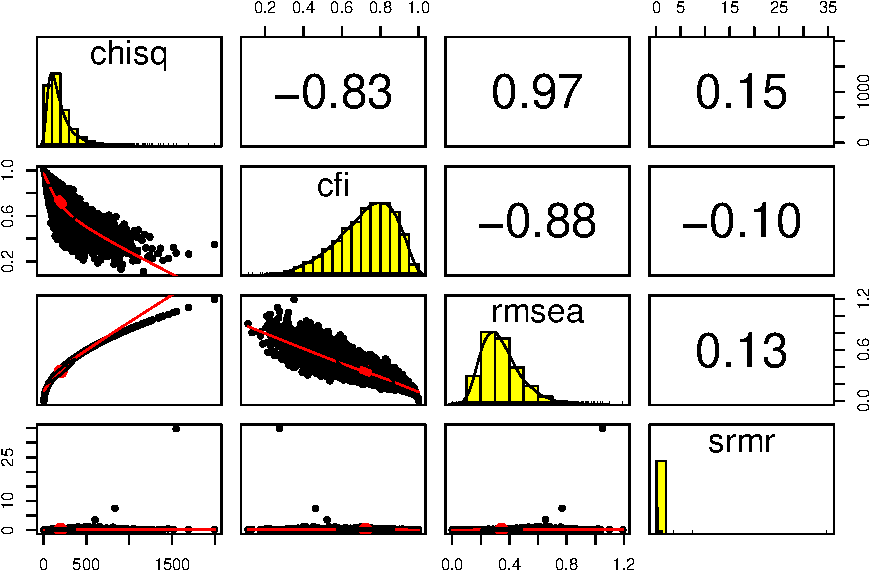
\includegraphics{Supplemental_materials_2_files/figure-latex/unnamed-chunk-7-1.pdf}

\begin{Shaded}
\begin{Highlighting}[]
\KeywordTok{save.image}\NormalTok{(}\StringTok{"SuppMat2.RData"}\NormalTok{)}

\KeywordTok{sessionInfo}\NormalTok{()}
\end{Highlighting}
\end{Shaded}

\begin{verbatim}
## R version 3.5.1 (2018-07-02)
## Platform: x86_64-pc-linux-gnu (64-bit)
## Running under: Ubuntu 18.04 LTS
## 
## Matrix products: default
## BLAS: /usr/lib/x86_64-linux-gnu/blas/libblas.so.3.7.1
## LAPACK: /usr/lib/x86_64-linux-gnu/lapack/liblapack.so.3.7.1
## 
## locale:
##  [1] LC_CTYPE=en_US.utf8       LC_NUMERIC=C             
##  [3] LC_TIME=en_US.utf8        LC_COLLATE=en_US.utf8    
##  [5] LC_MONETARY=en_US.utf8    LC_MESSAGES=en_US.utf8   
##  [7] LC_PAPER=en_US.utf8       LC_NAME=C                
##  [9] LC_ADDRESS=C              LC_TELEPHONE=C           
## [11] LC_MEASUREMENT=en_US.utf8 LC_IDENTIFICATION=C      
## 
## attached base packages:
## [1] stats     graphics  grDevices utils     datasets  methods   base     
## 
## other attached packages:
## [1] Matrix_1.2-14    psych_1.8.4      MASS_7.3-50      lavaan_0.6-1    
## [5] matrixcalc_1.0-3 plyr_1.8.4       rmarkdown_1.10  
## 
## loaded via a namespace (and not attached):
##  [1] Rcpp_0.12.17    knitr_1.20      magrittr_1.5    mnormt_1.5-5   
##  [5] pbivnorm_0.6.0  lattice_0.20-35 stringr_1.3.1   tools_3.5.1    
##  [9] parallel_3.5.1  grid_3.5.1      nlme_3.1-137    htmltools_0.3.6
## [13] yaml_2.1.19     rprojroot_1.3-2 digest_0.6.15   evaluate_0.10.1
## [17] stringi_1.2.3   compiler_3.5.1  backports_1.1.2 stats4_3.5.1   
## [21] foreign_0.8-70
\end{verbatim}


\end{document}
